\chapter{Fuzzy Logic}

\begin{chapquote}{Vladimir Ilyich Ulyanov}
``A lie told often enough becomes the truth.''
\end{chapquote}


\section{Basic concepts}

In the previous two chapters, we have been inquiring into
the issue of satisfiability of propositional calculus.
We expressed the notion of satisfiability by means of the
notions of truth and falsehood, that were represented
by the Scheme special values \texttt{\#t} and \texttt{\#f}.

It is customary however to represent these notions using
numerical values: truth is usually represented using $1$,
and falsehood -- using $0$. If we view it that way, the
conjunction can be perceived as a particular case of the
\textit{minimum} function, and disjunction -- as an
instance of the \textit{maximum} function. Furthermore,
the negation can be interpreted as the function $1-x$, where
$x$ is the logical value of the negated formula.

This observation could prompt someone to allow propositional
formulas to take any real value between $0$ and $1$, for
example $0.785398$, because then the basic junctions would
generalize naturally to support those values.

However unrealistic it may sound, this actually happened:
in the 1960s, Lotfi Zadeh proposed a theory of \textit{fuzzy
sets}, where the aforementioned observation found its
application. Unlike in the traditional set theory, where
a given element either belongs to a given set, or it does
not, Zadeh proposed a theory where an element can belong
to a set with a certain \textit{degree}, and each set
is characterized with a \textit{membership function}
that describes how certain elements (usually being real
numbers) belong -- or not -- to that set.

\section{Criticism}

Having formulated a theory, Zadeh tried to find an application
for it. Therefore he announced that his theory models the way
in which \textit{vague expressions} behave in the natural
language, and how people perform \textit{approximate reasoning}.

Worst of all, Zadeh really believed it. In the justification
of his work, he claimed that ``a natural language is basically
a system for describing perceptions''\cite{Zadeh2008}, not
even caring how is the sentence ``a natural language is basically
a system for describing perceptions'' a description of
a perception. Reading Zadeh's work, one gets the sense that,
trying to prove the value of his idea, he indeed started to
reason in a vague and imprecise way.

Among the examples that Zadeh gives is the notion of ``tallness''.
For example, most people will admit that a person that is
two-meters tall could be called a tall person. On the other
hand, if a person has $1.5$ meter, he will unlikely be called
a tall person. It is however impossible to set the limit between
the height to be considered tall and non-tall: we are more
likely to admit that the shift between tallness and non-tallness
occurs gradually.

Zadeh claims that the accurate description is to provide
a membership function that would describe the interpolation
between tallness and its negation.

The problem is that it is that there could be many competing
membership functions that differ only in some tiny details,
but there is no criterion to prefer any one of these functions
over another.

A deeper problem is that the whole ``thought experiment''
makes absolutely no sense: those seemingly ``vague''
descriptions usually serve the practical purpose
of designating an object of interest. We have no problem
understanding an expression ``the tall midget'' when
presented a group of midgets of varying height. But we
are rarely faced with the task of demarcating between
being tall and being non--tall.

Although the notion of fuzzy logic is very susceptible to
criticism that it has been receiving ever since it was
formulated, for some reason it also received a lot of attention
among people who dealt with Artificial Intelligence, and
some practical tools were built based on that theory
(It may be impressive to some that this actually succeeded,
but in practice the results were usually much less
efficient than they could be if the classical control
theory was applied).
Because of that, it will also be presented here, albeit
in a rather flaccid way.

\section{Exposition}

The remainder of this chapter will assume some basic
intuitions concerning real-valued functions of real variables.
The humanity won't suffer if you decide to skip it. (Make
however sure to read the section regarding the notion of 
\texttt{equivalence-classes}.)

Also, if you wish to get a detailed explanation of the presented
method, it's best if you look elsewhere.

We will use fuzzy logic to implement a virtual 
\textit{underwriter}, whose purpose is to give
a rating of potential clients for an insurance agency
based on a set of parameters, such as \textit{Body-Mass Index},
the level of \textit{glycated hemoglobin} in organism
or the \textit{blood pressure}.

The underwriter performs the inference based on a set
of \textit{fuzzy rules}, like ``if BMI is \textit{underweight}
or BMI is \textit{obese} or the glycated hemoglobin level is
\textit{low}, then the rating is \textit{refuse}''.

We could define the set of rules for the considered problem
in the following way.

\begin{Snippet}
(define underwriter-rules
  '((if (or (is bmi underweight) (is bmi obese)
            (is glycated-hemoglobin low))
	(is rating refuse))
    (if (or (is bmi overweight) (is glycated-hemoglobin low)
	    (is blood-pressure slight-overpressure))
	(is rating standard))
    (if (and (is bmi healthy) (is glycated-hemoglobin normal)
	     (is blood-pressure normal))
	(is rating preferred))))
\end{Snippet}

An inquisitive reader could ask an uncomfortable question:
why should we consider this set of rules as valid, rather
than some other one? The slack-off answer is that this
particular set was specified by an experienced professional
who encoded his or her intuitions acquired throughout the
years of practice.

Now we need to define what it means for the glycated hemoglobin
to be normal or low:

\begin{Snippet}
(define health-categories
  `((bmi (underweight ,(gaussian 9.25 3.0))
	 (healthy ,(gaussian 21.75 3.0))
	 (overweight ,(gaussian 27.5 3.0))
	 (obese ,(gaussian 35.0 3.0)))
    (glycated-hemoglobin (low ,(cone 4.0 5.0))
			 (normal ,(cone 5.25 5.0))
			 (high ,(cone 7.0 5.0)))
    (blood-pressure (normal ,(gaussian 0.0 2.5))
		    (slight-overpressure ,(gaussian 10.0 2.5))
		    (overpressure ,(gaussian 20.0 2.5))
		    (high-overpressure ,(gaussian 30.0 2.5)))
    (rating (refuse ,(cone 10.0 5.0))
	    (standard ,(cone 5.0 5.0))
	    (preferred ,(cone 1.0 5.0)))))
\end{Snippet}

An inquisitive reader could ask an uncomfortable question:
what makes us choose these shapes of membership functions
rather than some other ones? The slack-off answer would be
that the data was prepared and evaluated by a team of
highly educated medical experts who spent years studying
the complicated machinery of human body and now are able
to present their knowledge and linguistic intuitions
in a highly digestive form of a few functions of a single
variable. Even if you didn't trust that guy from the
insurance, it would be insane not to trust the medicals,
or wouldn't it?

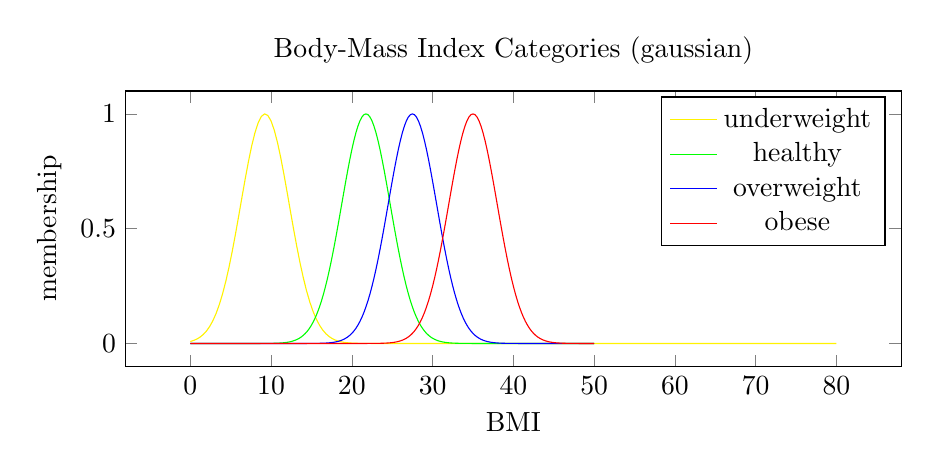
\begin{tikzpicture}
\begin{axis}[
    title=Body-Mass Index Categories (gaussian),
    xlabel=BMI,
    ylabel=membership,
    legend entries={underweight, healthy, overweight, obese},
    width = 4.5in,
    height = 2in
]
\addplot[ % underweight
yellow,
domain=0:80,
samples=201,
]
{exp(-(x-9.25)^2 / 18)};

\addplot[ % healthy
green,
domain=0:50,
samples=201,
]
{exp(-(x-21.75)^2 / 18)};

\addplot[ % overweight
blue,
domain=0:50,
samples=201,
]
{exp(-(x-27.5)^2 / 18)};

\addplot[ % obese
red,
domain=0:50,
samples=201,
]
{exp(-(x-35.0)^2 / 18)};

\end{axis}
\end{tikzpicture}

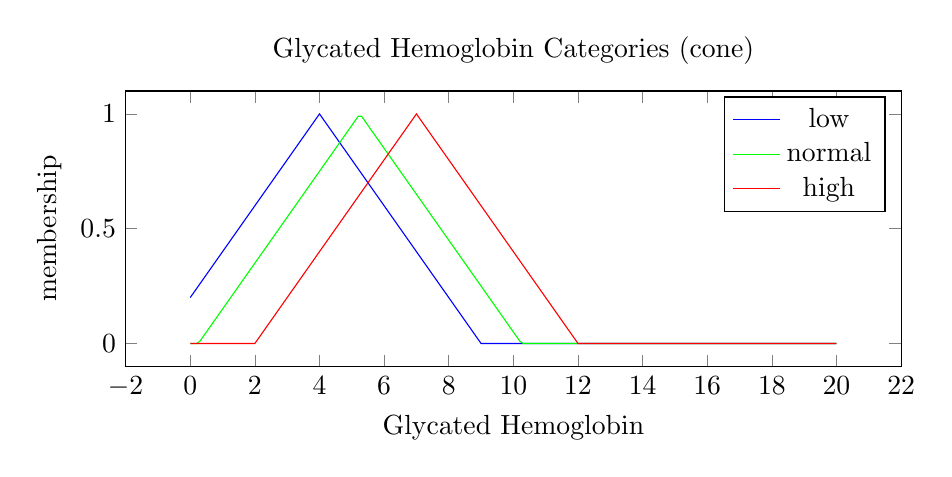
\begin{tikzpicture}[
  declare function={
    cone(\x) = and(\x>=-1,\x<0)*(\x+1) + and(\x>=0,\x<1)*(1-\x);
  }
]
\begin{axis}[
    title=Glycated Hemoglobin Categories (cone),
    xlabel=Glycated Hemoglobin,
    ylabel=membership,
    legend entries={low,normal,high},
    width = 4.5in,
    height = 2in
]
\addplot[ % low
blue,
domain=0:20,
samples=201,
]
{cone((x-4)/5)};

\addplot[ % normal
green,
domain=0:20,
samples=201,
]
{cone((x-5.25)/5)};

\addplot[ % high
red,
domain=0:20,
samples=201,
]
{cone((x-7)/5)};

\end{axis}
\end{tikzpicture}


It should be instructive to see the plots of at least some of
the membership functions, to appeal to our visual intuitions.
Also, for the practical purposes it is inevitable to define the
formulas for the cone and the gaussian curve:

\begin{Snippet}
(define ((gaussian center deviation) x)
  (exp (- (/ (square (- x center))
	     (* 2 (square deviation))))))
\end{Snippet}
\begin{Snippet}
(define ((cone center radius) x)
  (cond ((<= x (- center radius))
	 0)
	((<= x center)
	 (/ (+ x (- radius center)) radius))
	((< x (+ center radius))
	 (/ (+ (- x) center radius) radius))
	(else
	 0)))
\end{Snippet}

In the definition of \texttt{gaussian} we refer to the
built-in exponential function \texttt{(exp x)}, or $e^{x}$.

The definition of the \texttt{cone} function contains
a \texttt{cond} clause that we haven't seen before. It
is actually a variant of the \texttt{if} instruction
that we're already familiar with, and the definition
could as well have been written using the following form:

\begin{Snippet}
(define ((cone center radius) x)
  (if (<= x (- center radius))
    0
    (if (<= x center)
      (/ (+ x (- radius center)) radius)
      (if (< x (+ center radius))
        (/ (+ (- x) center radius) radius)
	0))))
\end{Snippet}

It is apparent that the form using \texttt{if}
has a more complex structure because of the
higher nesting level.

As all the rules and words' meanings are already known,
the only thing that's left is to actually conduct the
inference: given a tuple of labeled parameters describing
a \texttt{patient}, say, \texttt{((bmi 29) (glycated-hemoglobin 5)
(blood-pressure 20))}, we wish to provide a desired rating for it.
In other words, want to \texttt{(infer \#;from underwriter\--rules
\#;about patient \#;within health-categories)}.

First, we need to say to what \texttt{extent} does a
\texttt{patient} belong to a given classes: for example,
according to the membership functions defined above,
the BMI parameter of $29$ may be considered \textit{overweight}
with the degree $0.88$, \textit{obese} with the degree $0.13$,
\textit{healthy} with the degree $0.05$ and \textit{underweight}
with a degree very close to $0$.

So it would be convenient to have a function that, for
a given labeled tuple, returns the extent in which the
tuple's values belong to certain classes defined within
specified categories. It could also be handy if the classes
were sorted, so that the classes to which a given values
``belongs more'' would appear earlier on the list.

\begin{Snippet}
(define (extent #;in-which entity #;belongs-to categories)
  (map (lambda ((property value))
	 (let* ((category (lookup property categories))
		(classes (map (lambda ((name extent))
				`(,name ,(extent value)))
			      category)))
	   `(,property . ,(sort classes
				(lambda ((_ degree-1) (_ degree-2))
				  (> degree-1 degree-2))))))
       entity))
\end{Snippet}
\begin{Snippet}
(e.g.
 (extent '((bmi 29) (glycated-hemoglobin 5) (blood-pressure 20))
         health-categories)
 ===> ((bmi (overweight 0.8824969025845955) 
            (obese 0.1353352832366127) 
            (healthy 0.053926197030622854)
            (underweight 3.879522352578383e-10)) 
       (glycated-hemoglobin (normal 0.95) (low 0.8) (high 0.6)) 
       (blood-pressure (overpressure 1.0) 
                       (slight-overpressure 3.3546262790251185e-4) 
                       (high-overpressure 3.3546262790251185e-4)
                       (normal 1.2664165549094176e-14))))
\end{Snippet}

Probably the most surprising is the use of the \texttt{e.g.} form.
This is a syntactic extension that serves as a lightweight
\textit{unit test} framework: it evaluates the function before
the \texttt{===>} sign and raises an error condition it
its value isn't \texttt{equal?} to the value on the right.
It therefore enhances the reliability of the system, because
we have a confirmation that our function works as expected.

More importantly, it enriches the code with the information that
is more concrete and easier to digest than the sole definition,
because it shows exactly, which outputs can be expected for
given inputs.

The example could not be comprehended in the absence of
the definition of \texttt{health-categories}, but it shows
us what kind of output from the function we should expect,
which in turn prompts us with the idea of how this output
should be processed further.

We ought to take another look at our \texttt{underwriter\--rules}.
They all take the form 

\texttt{`(if ,condition (is ,property ,classification))}

where \texttt{condition} either has a form 

\texttt{`(is ,property ,classification)}

or is a junction (i.e. conjunction, disjunction or negation)
of simpler formulas. In the first case, say, 
\texttt{(is bmi overweight)} we evaluate it to the extent
in which the BMI belongs to the set ``overweight''.
In the particular case of BMI being equal $29$, it will
be the value of approx. $0.82$.

In the case of the junction of formulas, we evaluate
it according to the rules given above: conjunction
is the minimum function, disjunction -- the maximum
function, and negation -- the $1-x$ function.
Note the resemblance between the below
\texttt{satisfaction-degree} function and
the definition \texttt{satisfied?} from the earlier chapters.

\begin{Snippet}
(define (satisfaction-degree formula interpretation)
  (match formula
    (('and . clauses)
     (minimum (map (lambda (clause)
		       (satisfaction-degree clause interpretation))
		     clauses)))
    (('or . clauses)
     (maximum (map (lambda (clause)
		       (satisfaction-degree clause interpretation))
		     clauses)))
    (('not clause)
     (- 1.0 (satisfaction-degree clause interpretation)))
    (('is property classification)
     (let* ((classifications (lookup property interpretation))
	    ((extent) (lookup classification classifications)))
       extent))))
\end{Snippet}
\begin{Snippet}
;; where
(define (maximum list)
  (match list
    ((last)
     last)
    ((first . rest)
     (max first (maximum rest)))))

(define (minimum list)
  (match list
    ((last)
     last)
    ((first . rest)
     (min first (minimum rest)))))
\end{Snippet}

We defined two auxiliary functions that designate
the \texttt{minimum} and \texttt{maximum} of the list,
using the built-in \texttt{min} and \texttt{max}
functions that return the largest of its arguments.
As we will see in the following chapters, that definition
wasn't strictly necessary.

Now that we can determine the \texttt{satisfaction-degree}
of a given predicative formula, we have a set of rules
and the preconditions of those rules, the only thing
that is left is to conduct the inference.

This is actually the trickiest part, as it is concerned
with a notion (or rather pseudo-notion) of \textit{defuzzification}.
Let me remind that the \texttt{underwriter\--rules} consist
of three rules, corresponding to three possible classifications
of \texttt{rating}: \texttt{standard}, \texttt{perfect} and
\texttt{refuse}. For example, the first rule said:

\begin{Snippet}
(if (or (is bmi underweight) (is bmi obese)
        (is glycated-hemoglobin low))
    (is rating refuse))
\end{Snippet}


We need to blend those three rules, based on the extents
of their preconditions, in order to choose the ``right''
classification.

One idea would be to choose the rule whose precondition
is the highest \texttt{satisfaction-degree}. However, according
to Wikipedia, ``this approach loses information''. Therefore
another method is used: first we clip the membership functions
for the various classes of the category \texttt{rating}, so that
their values are limited to the satisfaction-degrees, then
we create a new function that gives the maximum of each of the
clipped functions, and finally we apply some numerical method
like calculation of the \textit{center of gravity} of the function
(Wikipedia lists 20 other defuzzification functions, each of them being
equally arbitrary, none of them having any apparent advantages
over the another).

\begin{Snippet}
(define (infer #;from rules #;about entity #;within categories)
  (let* ((judgment (extent entity categories)) 
	 (conclusions 
          (map
           (lambda (('if condition ('is property classification)))
             (let* ((degree (satisfaction-degree condition judgment))
                    (categories (lookup property categories))
                    ((membership) (lookup classification categories))
                    (conclusion (clip membership 0 degree)))
               `(,property ,conclusion)))
           rules))
	 (common-subject (equivalence-classes 
			  (lambda ((property-1 _) (property-2 _))
			    (eq? property-1 property-2))
			  conclusions)))
    (map (lambda (((properties functions) ...))
	   (let* (((property . _) properties)
		  (composition (lambda (x)
		 		 (maximum (map (lambda (f) 
                                                 (f x))
                                               functions)))))
	     `(,property ,composition)))
	 common-subject)))
\end{Snippet}

The code above is somewhat terse, and requires a bit of explanation.
First we calculate the \texttt{judgment} using the \texttt{condition}
function. The \texttt{judgment} therefore contains a list of the
form \texttt{'((bmi (overweight 0.9) (normal 0.1) ...)
(glycated-hemoglobin (normal 0.9) ...) ...)}. Then for each rule
we decompose it into \texttt{condition} and the consequent of the form
\texttt{('is property classification)}, so for example, the name
\texttt{condition} can be bound to the sequence 
\texttt{'(or (is bmi underweight) (is bmi obese) 
(is glycated-hemoglobin low))},  \texttt{property} is bound to 
\texttt{'rating}, and \texttt{classification} is bound to 
\texttt{'refuse}. Then we take the \texttt{membership} function
for the given \texttt{property} and \texttt{classification} pair.
In the case of \texttt{rating}, \texttt{refuse} it is the 
\texttt{(cone 10.0 5.0)} function. Eventually we return a pair with
the name of the classification and the clipped membership function.

Note that although it isn't the case with our example, we could in
general have more properties than just \texttt{rating} contained
in the consequents of our rules. Therefor we would need to split
the rules that refer to the same property. This is what the
\texttt{equivalence-classes} concept is for. In general, it takes
a set and the so-called \textit{equivalence relation}\footnote{
Intuitively, an equivalence relation expresses some sort of common
property, like ``$X$ is of the same religion as $Y$''. This
particular relation divides humans into equivalence classes such
as Buddhists, Christians, Jews, Muslims, and so on, which
leads to many pointless wars.} and returns a list of lists whose
elements all belong to the same equivalence class.

For example, if we had a list of natural numbers, say,
\texttt{(1 2 3 4 5 6 7 8 9)}, then its equivalence classes
for the equivalence relation ``$x$ and $y$ have the same
remainder of the division by $3$'' would be a list of three
lists: \texttt{((1 4 7) (2 5 8) (3 6 9))}.

Although the notion of \texttt{equivalence-classes} isn't essential
for this particular task, it will be used later, so I will present
the code here without any comments, except the note that it preserves
the original order among the elements of the classes, and the
observation that it uses the so-called \textit{named-let} construct
that won't be covered in this pamphlet. The explanation isn't
difficult to find with Google.

\begin{Snippet}
(define (equivalence-classes equivalent? set)
  (let next-item ((set set)(result '()))
    (match set
      (()
       (reverse (map reverse result)))
      ((item . set)
       (match result
	 (()
	  (next-item set `((,item) . ,result)))
	 ((this . next)
	  (let next-class ((past '()) (present this) (future next))
	    (match present
	      ((paradigm . _)
	       (if (equivalent? item paradigm)
		   (next-item set `((,item . ,present)
				    . (,@past ,@future)))
		   (match future
		     (()
		      (next-item set `((,item) ,@result)))
		     ((this . next)
		      (next-class `(,present . ,past) this next)))
                    )))
             )))))))
\end{Snippet}

Having the conclusions split into \texttt{equivalence-classes}
of conclusions that regard the same \texttt{property}, we create
a \texttt{composition} of the clipped functions of \texttt{membership}
to given \texttt{classification}s, which are constructed by
selecting the \texttt{maximum} value of each of the component
functions.

The only thing that may be unknown at this point is what it means
to \texttt{clip} a function. This is rather straightforward:

\begin{Snippet}
(define ((clip function bottom top) x)
  (assert (<= bottom top))
  (max bottom (min top (function x))))
\end{Snippet}

The \texttt{infer} function returns a list of form
\texttt{((property function) ...)}. In order to get
the classifications of the \texttt{property} values,
we need to defuzzify each \texttt{function}.

We are going to use the aforementioned method of
computing the \texttt{center\--of\--gravity}. This
method is based on \textit{numerical integration}
that will not be covered here.

\begin{Snippet}
(with-default ((bottom 0)
	       (top 100)
	       (step 0.1))
  (define (center-of-gravity function)
    (let* ((step (specific step))
	   (domain (range #;from (specific bottom) 
				#;to (specific top) #;by step)))
      (/ (sum (map (lambda (x) (* x (function x) step)) domain))
	 (sum (map (lambda (x) (* (function x) step)) domain))))))
;; where
(define (range #;from bottom #;to top #;by step)
  (if (> bottom top)
    '()
    `(,bottom . ,(range #;from (+ bottom step) #;to top #;by step))))
\end{Snippet}

The surprising thing is the use of the \texttt{with-default} derived
form. It is used to give some default values to certain names,
but without committing to those values. The form will be explained
in one of the later chapters.

Finally, we can evaluate the expression

\begin{Snippet}
(let* ((conclusions (infer #;from underwriter-rules 
				  #;about '((bmi 29) 
					    (glycated-hemoglobin 5) 
					    (blood-pressure 20))
				  #;within health-categories)))
  (map (lambda ((property function))
	 `(,property ,(center-of-gravity function)))
       conclusions))
\end{Snippet}

to find out that the \texttt{rating} received by our candidate is $7.46$.
In other words, we passed along some numbers to receive yet another number.
